\chapter{Plataforma de desarrollo}
\label{cap:capitulo3}

\begin{flushright}
\begin{minipage}[]{10cm}
\emph{Quizás algún fragmento de libro inspirador...}\\
\end{minipage}\\

Autor, \textit{Título}\\
\end{flushright}

\vspace{1cm}

En este capítulo, se explica el hardware y software elegido para desarrollar el trabajo y los motivos de dicha elección.

\section{Hardware}
\subsection{\textit{NVIDIA Jetson Nano}}
La placa de desarrollo \textit{NVIDIA Jetson Nano} es una plataforma de bajo coste con grandes capacidades computacionales para implementar técnicas de inteligencia artificial gracias a su \textit{GPU} dedicada \textit{NVIDIA Maxwell} con 128 \textit{NVIDIA CUDA cores}, además dispone de una CPU Quad-core basada en la arquitectura Aarch64 lo que permite ejecutar GNU/Linux sin dificultades y ser compatible con numerosas bibliotecas de código. La placa en cuestión, dispone además de pines GPIO lo que permite de forma muy sencilla conectar todo tipo de sensores y actuadores.\\

Los requisitos en lo que a alimentación se refiere no son excesivos, requiere un mínimo de 5 voltios y 3 amperios, lo que permite que una simple \textit{powerbank} de reducido tamaño sea capaz de alimentar la placa, si bien es cierto que la batería debe poder ofrecer tres amperios de forma estable, y no solo como intensidad pico. Existen numerosos proyectos en los que esta placa está presente, tales como JetBot o JetRacer.\\

\begin{figure} [h!]
	\begin{center}
		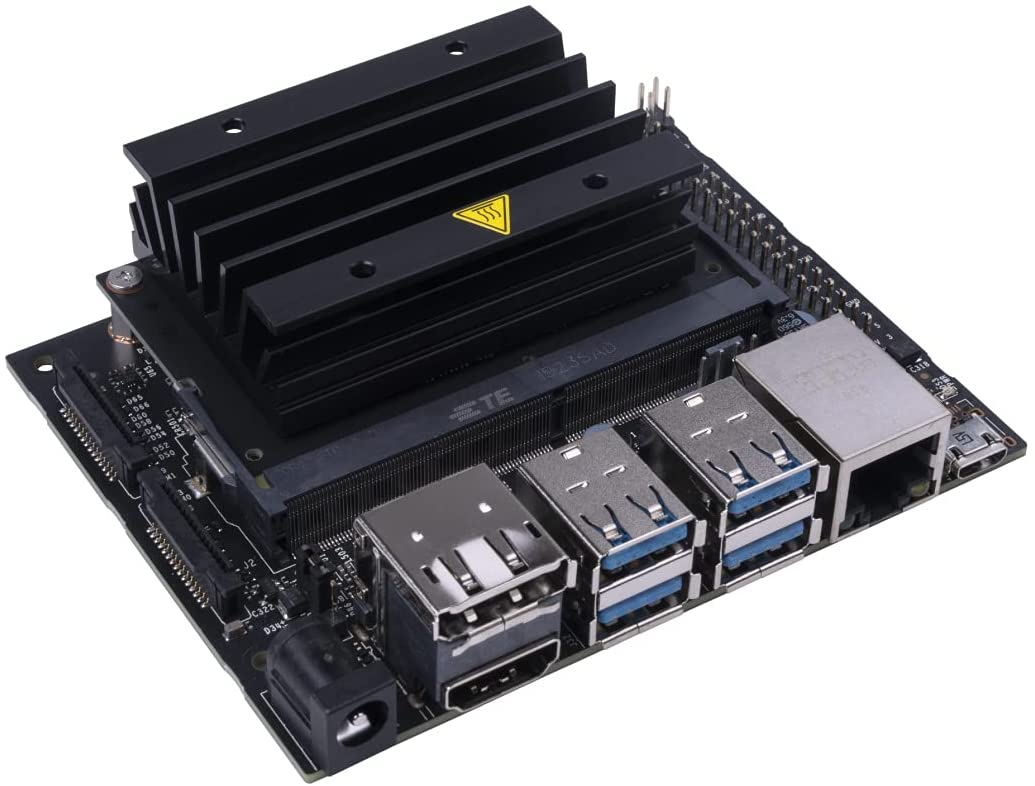
\includegraphics[width=6cm]{figs/jetsonnano}
	\end{center}
	\caption{\textit{NVIDIA Jetson Nano}.}
	\label{fig:jetsonnano}
\end{figure}\

https://developer.nvidia.com/embedded/jetson-nano

\subsection{Motores \textit{TT}}
Se trata de unos motores de corriente continua con reductora utilizados en la multitud de proyectos de robótica de bajo coste cite cite. La tensión de alimentación tiene un rango de 3 a 6 voltios y la velocidad mínima en vacío tiene un rango de 90 a 200 revoluciones por minuto dependiendo del voltaje, lo que permite conseguir una velocidad reducida para robots de pequeño tamaño.\\ 

\begin{figure} [h!]
	\begin{center}
		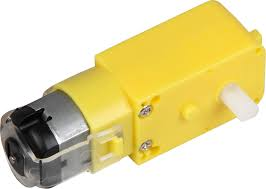
\includegraphics[width=6cm]{figs/motorTT}
	\end{center}
	\caption{Motores \textit{TT}.}
	\label{fig:motorTT}
\end{figure}\

https://www.verical.com/datasheet/adafruit-brushless-dc-motors-3777-5912007.pdf


\subsection{Controladora de motores \textit{L298N}}
Es un módulo capaz de controlar la dirección y la velocidad de los motores anteriormente citados. La tensión de alimentación es de un mínimo de 6 voltios, lo que hace imposible alimentarla con la placa \textit{NVIDIA Jetson Nano} por lo que es necesario una batería externa. Otra posibilidad para utilizar una única batería sería utilizar la salida de 5 voltios (V) que nos ofrece la controladora, sin embargo, dicha salida nunca ofrecerá los 3 amperios (A) requeridos. Este componente permite invertir el sentido de la corriente lo que proporciona un control para mover los motores en el sentido de las agujas del reloj (CW) y en el sentido contrario a las agujas del reloj (CCW). La principal limitación de esta placa es que solo permite controlar dos motores, por lo que si se dispone de 4 motores, se podrán conectar a pares dependiendo del comportamiento deseado. El control se realiza a través de la técnica PWM, que permite enviar de forma precisa la velocidad deseada a través de una señal digital.\\

\begin{figure} [h!]
	\begin{center}
		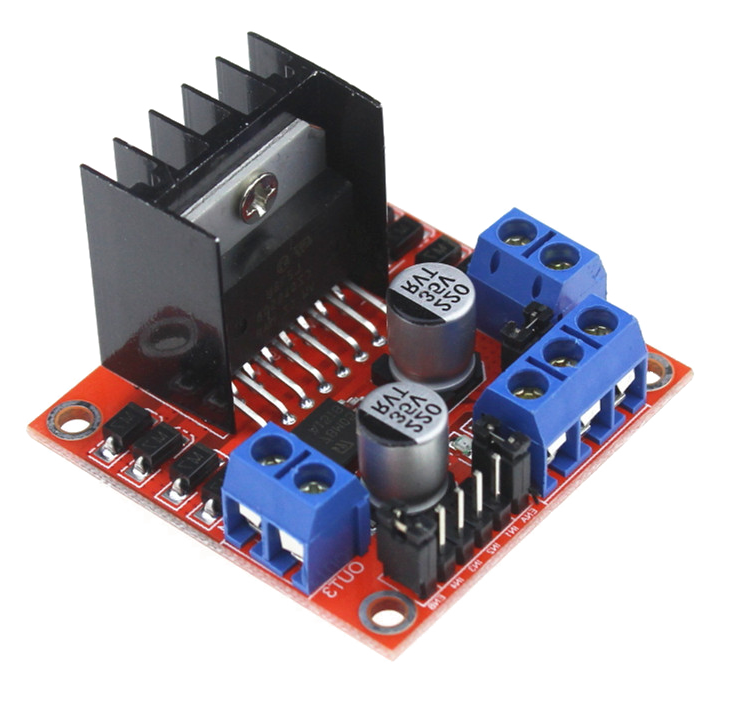
\includegraphics[width=6cm]{figs/l298n}
	\end{center}
	\caption{Controladora de motores \textit{L298N}.}
	\label{fig:l298n}
\end{figure}\

https://www.luisllamas.es/arduino-motor-corriente-continua-l298n/

\subsection{Cámara \textit{Xiaomi}}
Se trata de una cámara USB lo que permite recibir la imagen a través de dicho puerto con una tasa de 30 \textit{frames} por segundo (FPS). Su resolución es 1080p pero permite obtener una imagen de menor resolución a través de su driver.\\

\begin{figure} [h!]
	\begin{center}
		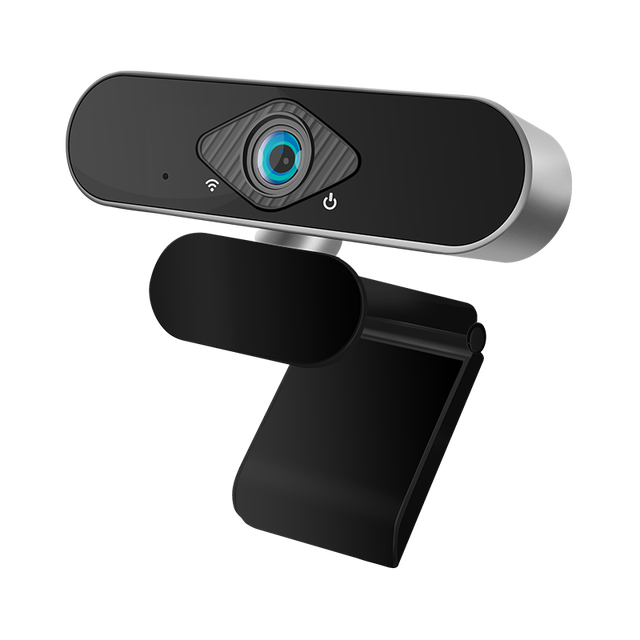
\includegraphics[width=6cm]{figs/camera}
	\end{center}
	\caption{Cámara \textit{Xiaomi}.}
	\label{fig:camera}
\end{figure}\

\subsection{Batería 10000mAh}
Su capacidad es de 10000 miliamperios hora (mAh), el voltaje de funcionamiento es 5 voltios (V) y su intensidad teórica es 3 amperios (A) por lo que permite alimentar la placa \textit{NVIDIA Jetson Nano}.\\


\begin{figure} [h!]
	\begin{center}
		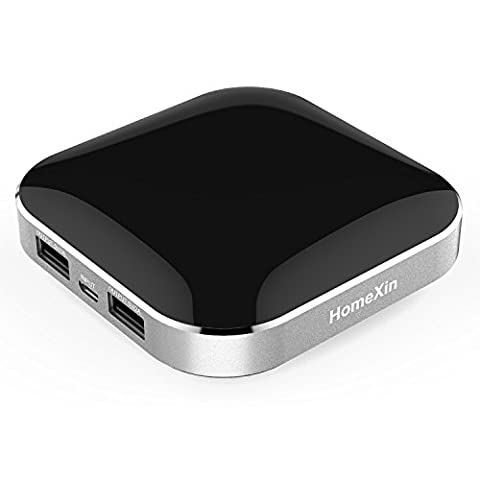
\includegraphics[width=6cm]{figs/battery}
	\end{center}
	\caption{Batería 10000mAh.}
	\label{fig:battery}
\end{figure}\

\subsection{Chasis}
Se trata de un chasis de bajo coste muy común en proyectos relacionados con Arduino. Dispone de soportes para los motores TT cite, lo que perimite ensamblarlos de forma muy sencilla. El tamaño es suficiente para alojar todos los componentes elegidos utilizando los agujeros predefinidos en el chasis.\\

\begin{figure} [h!]
	\begin{center}
		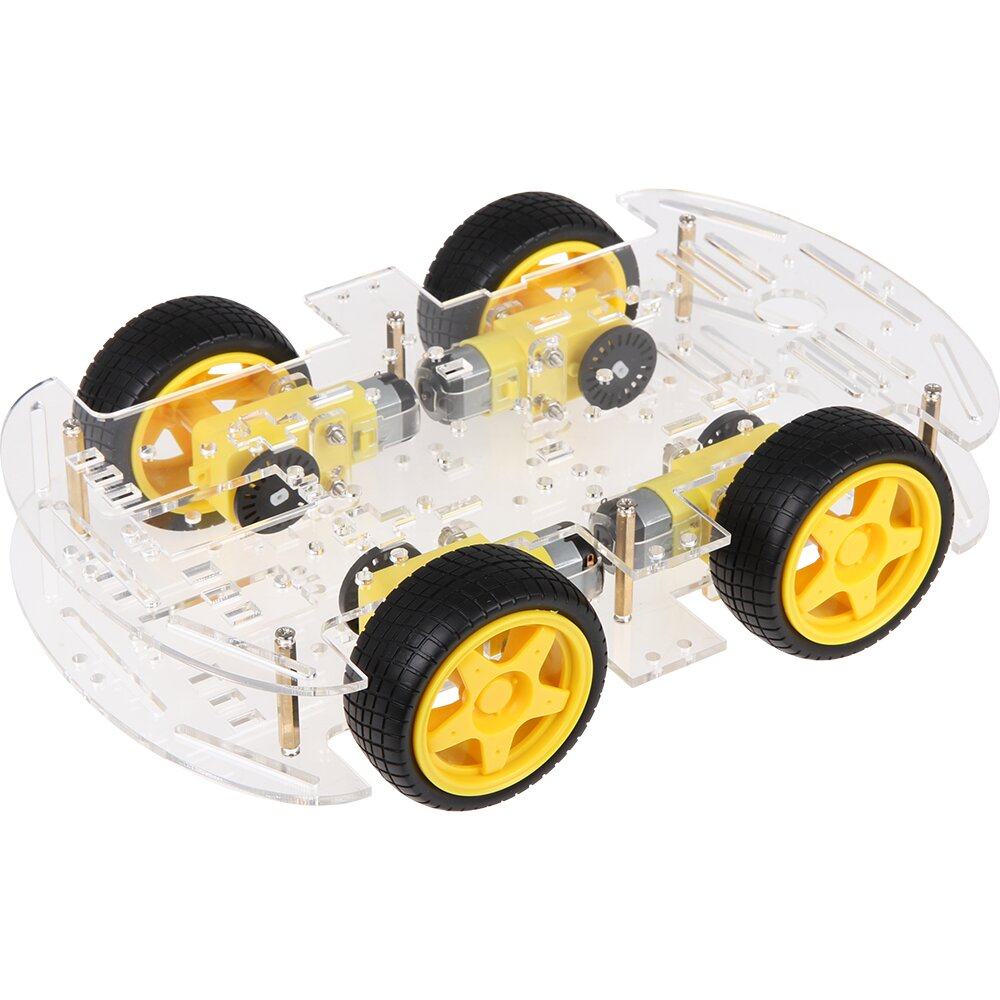
\includegraphics[width=6cm]{figs/chasis}
	\end{center}
	\caption{Chasis.}
	\label{fig:chasis}
\end{figure}\

\section{Software}

\subsection{\textit{Python}}
Python es un lenguaje de programación de código abierto, interpretado, orientado a objetos y de alto nivel. En la actualidad es el lenguaje más usado a nivel mundial cite. Está considerado como un lenguaje fácil de aprender gracias a su simple sintáxis, esto le ha llevado a crecer mucho en popularidad durante los últimos años. Además, al ser interpretado, no es necesario utilizar un compilador, lo que provoca un desarrollo mucho más rápido. Python cuenta con una enorme cantidad de bibliotecas y clientes para utilizar software desarrollado en otros lenguajes. Algunas de ellas se describirán a continuación. 


https://pypl.github.io/PYPL.html
\subsection{\textit{Blender}}

\subsection{\textit{Gazebo}}
\textit{Ignition Gazebo} es un simulador 3D de código abierto desarrollado por la \textit{Open Source Robotics Foundation (OSRF)}, escrito en \textit{C++}, usado principalmente para simular comportamientos con gran precisión y gráficos de alta calidad en los que intervienen robots en un entorno dinámico. Desde  Utiliza, por defecto, el motor de físicas \textit{ODE} cite, escrito también en \textit{C++}. Permite simular todo tipo de sensores y actuadores. Además, ofrece integración con ROS de forma muy sencilla. 

https://www.openrobotics.org/
https://github.com/gazebosim/gz-sim
https://bitbucket.org/odedevs/ode/src/master/

\subsection{\textit{ROS}}
Robot Operating System \textit{ROS} es un middleware róbotico, de código abierto, con multitud de bibliotecas y herramientas desarrollado por la \textit{Open Source Robotics Foundation (OSRF)}, escrito en \textit{C++} y \textit{Python}. Es considerado actualmente el estándar en robótica. Permite desarrollar aplicaciones complejas en las intervienen diversos procesos llamados nodos, que se comunican entre ellos mediante \textit{topics} y servicios. Una de las principales ventajas de utilizar un middleware como ROS es la capacidad de abstracción que proporciona, de forma que el usuario únicamente programa sobre una interfaz dada, disponible en \textit{C++} y \textit{Python}, sin preocuparse por lo que pasa por debajo.

https://www.openrobotics.org/
http://wiki.ros.org/Nodes
http://wiki.ros.org/Topics
http://wiki.ros.org/Services
http://wiki.ros.org/Client%20Libraries

\subsection{OpenCV}
OpenCV es una librería de visión artificial de código abierto desarrollado por Intel. Está escrita en \textit{C/C++} y cuenta con soporte para aceleración por GPU basadas en CUDA y OpenCL y procesamiento de imagen en tiempo real. Es usada en todo tipo de aplicaciones en las que interviene la visión por ordenador, tales como, detección de objetos, realidad aumentada o reconocimiento de gestos. Además, está disponible en multitud de lenguajes de programación; \textit{C++}, \textit{Python}, \textit{Java}, etc...

https://opencv.org/opencv-platinum-membership/
https://github.com/opencv/opencv

\subsection{Darknet}
Darknet es un framework de código abierto que permite ejecutar y entrenar redes neuronales en tiempo real, ya que soporta tanto computación por CPU como GPU. Está escrito en C y CUDA, gracias a estar escrito en un lenguaje considerado de bajo nivel, ofrece un rendimiento aceptable en plataformas de bajo coste como cite jetson.
https://pjreddie.com/darknet/

\subsection{PyQt}

\subsection{JetRacer}
PyTorch, PyTorch to TensorRT y Torchvision



Mapa 